% ---- ETD Document Class and Useful Packages ---- %
\documentclass{ucetd}
\usepackage{subfigure,epsfig,amsfonts}
\usepackage{natbib}
\usepackage{amsmath}
\usepackage{amssymb}
\usepackage{amsthm}

\usepackage{graphicx}
\graphicspath{{Figures/}}
\usepackage{color}
\usepackage{listings}
% set the default code style
\lstset{
    frame=tb, % draw a frame at the top and bottom of the code block
    tabsize=4, % tab space width
    showstringspaces=false, % don't mark spaces in strings
    numbers=left, % display line numbers on the left
    commentstyle=\color{green}, % comment color
    keywordstyle=\color{blue}, % keyword color
    stringstyle=\color{red} % string color
}

\usepackage[toc,page]{appendix}

%% Use these commands to set biographic information for the title page:
\title{Exploring higher-order relationships in microbial protein networks}
\author{Rida Assaf}
\department{Computer Science}
\division{Physical Science Division}
\degree{Master of Science}
\date{April 01, 2015}

%% Use these commands to set a dedication and epigraph text
\dedication{Dedicated to}
\epigraph{Epigraph Text}


\begin{document}
%% Basic setup commands
% If you don't want a title page comment out the next line and uncomment the line after it:
\maketitle
%\omittitle

% These lines can be commented out to disable the copyright/dedication/epigraph pages
\makecopyright
\makededication
\makeepigraph


%% Make the various tables of contents
\tableofcontents
\listoffigures
%\listoftables

\acknowledgments
% Enter Acknowledgements here

\abstract
% Enter Abstract here
With the advancement in genome sequencing technology and the ever-growing set of fully sequenced genomes made available to researchers,  genomic context analysis has attracted much interest. Investigating protein networks is a major focus of genome research, and the methods used to predict these interactions have been put on a quantitative basis. That is because they have been shown to be equally effective to experimental methods. Among the various methods that have been proposed to predict functional interactions between proteins based on the genomic context of their genes, we focus our attention to phylogenetic profiling methods which link proteins based on the high correlation between their phyletic distributions across a set of genomes. One of the goals of this research is to discover novel pathways in meta-genomic datasets. 
We show examples of current tools on the web that provide similar functionalities but are limited by some factors.  We present our methods that alleviate some of these limitations and demonstrate their effectiveness by predicting a well-known pathway. 

\mainmatter
% Main body of text follows

\chapter{Introduction}
% Introductory stuff
Studying the networks of molecular interactions that underlie cellular function is a  major focus of genome research\cite{1}. The methods used to predict these interactions have been put on a quantitative basis. That is because since they seem to be at least on an equal footing with genomics experimental data, the thing that was shown by a survey of experimentally confirmed predictions\cite{4}. The sequencing of genomes from different species made it possible not only to get a consensus of all proteins but also to analyze their functions. \cite{1, 10,11,12,13,14,15}. The abundance of fully sequenced genomes and high throughput algorithms in comparative genomics created the opportunity to predict functionally linked proteins and to transfer the functionality of annotated proteins to un-annotated ones \cite{8}. Context-based function prediction is complementary to homology-based function prediction\cite{5, 17}. For a given protein, homology-based methods predict the molecular function of that protein, whereas context-based methods may predict a higher order function like what other proteins it interacts with or which pathway it plays a role in \cite{5}.  Other than direct physical binding, proteins may also interact indirectly. Examples of indirect interactions are sharing a substrate in a metabolic pathway, regulating other  proteins transcriptionally, or forming multi-protein assemblies \cite{6, 18,19,17}. The use of Protein networks is not limited to the increase of statistical power in human genetics\cite{21,22}, but extends to aiding in drug discovery\cite{23,24}, closing gaps in metabolic enzyme knowledge\cite{25,26}, and predicting phenotypes and gene functions\cite{3, 27,28}. 
Among the various methods that have been proposed to predict functional interactions between proteins based on the genomic context of their genes are phylogenetic profiling methods and the domain fusion method\cite{5}. Given a set of fully sequenced genomes, phylogenetic profiling methods link proteins based on the high correlation between their phyletic distribution across that set \cite{29, 30, 31}. Whereas the domain fusion method identifies protein pairs that fuse into a single peptide in another organism \cite{8, 32, 33}.  Another method makes use of the observation that potential operons(genes that fall in each other's proximity on genomes) encode functionally interacting proteins. \cite{2, 35,36,37,38,39}.  The method we adopt in this thesis is the phylogenetic profiling approach \cite{1, 40, 41, 42} that detects functional relationships between proteins that show statistically similar patterns of presence or absence. Given a protein, we can search for its homologs across the different sequenced genomes in our database to determine the pattern describing its absence or presence. We can represent that pattern as a vector, storing 1 where a protein is present and 0 otherwise. This vector is referred to as the phylogenetic profile of that protein. Original implementations of the phylogenetic profile method considered proteins with similar profiles to be potentially functionally related \cite{40}.  Other ideas suggest that proteins may be linked if their profiles represented the negation of each other \cite{43, 44}. 
These ideas represent a simple relation between two proteins in a cell, with the presence of one protein affecting the presence or absence of the other. The simplicity of such patterns might be limited to cases when two proteins are required to form a structural complex or when two proteins carry out sequential steps in an un-branched metabolic pathway. In order to describe the full complexity of cellular networks that involve branching, parallel, and alternate pathways, we expect the existence of higher order logic relationships involving a pattern of presence or absence of multiple proteins\cite{1}.

Other than inferring protein networks that might help us understand protein functions and figuring out what genes are associated with each other, among the many reasons why we care about genomic context analysis is hoping to devise a way that would aid in the discovery of novel pathways in meta-genomic datasets.  We are also interested in having a way to estimate operons and their occurrence in given genomes, in addition to finding out protein or gene co-occurrences that are signatures of a given clade or genera. The implications of such discoveries would be tremendous and take us steps forward towards unmasking more mysteries in the biology domain. 
The rest of this paper is organized as follows, first we present some background of the statistical tools we used in this work. Then, we present some previous work in the literature, and show what of these questions they have tackled and where their limitations lie. Then, we present our work that presents new robust methods to answer some of these questions, and alleviate some limitations the current work in the literature has. We present our results and findings along the way, and finish with some concluding remarks. 


\chapter{Background}
%%\section{Introduction}
% Intro to chapter one
One way to evaluate the correlation between two proteins is by calculating their conditional probability. The probability of seeing  protein X given the probability of seeing protein Y is defined by:

\begin{center}
$P(X|Y) = \frac{P(X,Y)}{P(Y)}$\\
\end{center}
In the event that P(X,Y) = P(X)P(Y) or P($X|Y$) = P(X), X and Y are considered to be independent. Else, X and Y are correlated. \\

The mutual information also provides a score for the co-occurrence of two genes. It is maximal when both genes occur in about 50\% of the genomes (the individual entropies of the genes are maximal) and the genes occur always together (the combined entropy is minimal)\cite{5}.\\
Mutual Information can be defined as: 

\begin{center}
$MI(X,Y) = H(X,Y) - H(X|Y) - H(Y|X)$\\
\end{center}
Where H(X) and H(Y) are the marginal entropies, H($X|Y$) and H($Y|X$) are the conditional entropies, and H(X,Y) is the joint entropy of proteins X and Y. 
Another identity of the Mutual Information of proteins X and Y can be defined as:

\begin{center}
$MI(X,Y) = \sum\limits_{y\in Y}\sum\limits_{x\in X}p(x,y)log\left(\frac{p(x,y)}{P(x)(P(y)}\right)$

\end{center}
Where p(x,y) is the joint probability distribution function of X and Y, and p(x) and p(y) are the marginal probability distribution functions of X and  Y respectively. \newpage

Note that using genomic-context methods to design an experiment based on scores obtained using any of the two metrics mentioned above is not that trivial. This is because these methods may predict an interaction between proteins, but they do not predict the type of  that interaction. For example, in the case of a metabolic pathway, these methods may tell us that a protein belongs to a certain pathway, but they do not say where in that pathway we can place the hypothetical protein. 
One way to increase the prediction specificity is to take the evolutionary conservation of a genomic-context pattern into account. For example, the more often that the genes occur in each other's proximity, the more likely that the proteins they encode functionally interact in the most direct way \cite{4, 45}. 
Gene clusters are known to be prominent features of bacterial chromosomes. Demerec and Hartman postulated in 1959 that ``regardless of how the gene clusters originated, natural selection must act to prevent their separation'' and the ``mere existence of such arrangements shows that they must be beneficial, conferring an evolutionary advantage on individuals and populations which exhibit them.'' \cite{7}.





\chapter{Literature Review}
LAPP(logic analysis of phylogenetic profiles) is a computational approach for identifying detailed relationships between proteins on the basis of genomic data. Logic analysis of phylogenetic profiles identifies triplets of proteins whose presence or absence obey certain logic relationships. For example, protein C may be present in a genome only if proteins A and B are both present\cite{1}. 
There are eight possible logic relationships relating two phylogenetic profiles to another. By calculating the uncertainty coefficients and using Mutual Information, the authors uncovered 750,000 new protein relationships for triplets where the individual pairwise uncertainty scores of the first two proteins described the third poorly but the logically combined profile described it well. (In other words: $H(Z|X)<0.3$ and $H(Z|Y) < 0.3$ but $H(Z|(X,Y)) > 0.6$) where X,Y, and Z are the proteins of interest and H is the uncertainty score used in the Mutual Information equation.
Different tools on the web provide different services for genomic context analysis. 
N-Browse takes a seed gene as an input and returns all those related to it. I2D takes one protein at a time and gives known and predicted mammalian and eukaryotic protein-protein interactions. BioPixie is a system for analysis and visualization of biological network predictions in S. Cerevisiaie. Given a protein or group of proteins as a query set (the expert-driven search component), a novel probabilistic algorithm considers the integrated pair-wise relationships to build a local process-specific network around the query proteins. Even though these tools provide some insight about protein functionality and correlation, we are usually interested in higher order relationships and more than pairwise correlation between them as previously mentioned. We are also interested in exploring protein networks from recovered meta-genomic data and prokaryotes. A tool that alleviates this limitation is GeneMANIA, that takes as input a query of seed genes(not limited to 1), and returns the genes that are related to them. One problem with these tools however, is that they only return the genes/proteins that are directly related to the query ones. We are often interested in the set of genes/proteins that are indirectly related to our query genes/proteins as well, as this may uncover a broad set of new functional correlation and help us gain a better understanding of pathways. A tool that helps with that is VisANT, which starts from an initial gene/drug of interest, and uses exploratory navigation that allows you to walk through the interactions one by one. The interactions between genes are either physical or genetic, and the interactions between genes and drugs indicate the corresponding binding targets of the drugs(takes one at a time, and shows hierarchy). 
A tool that is somehow different is APID(Agile Protein Interaction DataAnalyzer), which helps analyze known information about protein-protein interactions that have been demonstrated by experimental methods.   
Some of these tools have limitations that are alleviated by others, like being able to provide only pairwise information, or only the directly related genes/proteins. 

	Now we discuss a tool that we believe offers a wider array of functions that are of interest in our research. STRING (search tool for recurring instances of neighboring genes) is a tool to retrieve and display the genes a query gene repeatedly occurs with in clusters on the genome\cite{2}. STRING also retrieves genes that are indirectly(via other genes) related to the query gene. STRING takes a seed gene as input, gets all genes that match it, and treats these as seed genes in the next iteration. The process repeats until the number of iterations specified by the user is reached or until no new genes are found(convergence)\cite{2}. Associations in STRING are provided with a probabilistic confidence score, which is derived by separately benchmarking groups of associations against the manually curated functional classification scheme of the KEGG database \cite{46}.
All scores and association data in STRING are pre-computed\cite{3}. Which might explain why it only supports queries for a single gene/protein at a time and thus does not offer a way to investigate higher dimension relationships. 

	Moreover, one limitation all these tools have in common is the lack of support for negated variables as input. In other words, sometimes we are interested in studying the implications of the absence of one protein on the presence/absence of others, especially when that protein is part of a larger input vector of interest. However, none of the mentioned tools or any others that we know of provides this functionality. 

	As we mentioned before, one of the things we are interested in is discovering novel pathways. Two interesting tools that try to offer this functionality are LPAT(Linear Pathfinding with Atom Tracking) and SPABBATS. LPAT is an algorithm for finding atom conserving linear pathways in metabolic networks. LPAT takes as input a start compound, a target compound, the minimum number of atoms to be conserved, the number of pathways to return, k, and a special data structure, termed an atom mapping graph. LPAT is then guaranteed to return the k shortest pathways between the start and target compounds that conserve at least a given number of atoms.
SPABBATS is an algorithm based on Boolean satisfiability (SAT) that computes alternative metabolic pathways between input and output species in a reconstructed network.
In our journey of discovering novel pathways, we do not want to limit ourselves by having to specify the input and the target. What would be more interesting is having a map of different possible interactions that lead to an end result, and traversing that map to see what targets might be of interest and what input can lead to these targets. We find that to be a closer definition of novelty. 

	These tools and methods may help us infer protein networks, predict protein functions, gene associations, and novel pathways, but the help they offer is very limited. Besides, there is no obvious way in which we can use these tools to estimate operons and their occurrence in given genomes, or to find out protein or gene co-occurrences that are signatures of a given clade or genera. Thus, in the rest of paper, we present the approaches we took to alleviate some of these tools' limitations, and take a step further in answering a wider range of questions. 
	
\chapter{Methods}
	One way to think about the problem of getting the set of proteins that are potentially related to a query protein is by thinking about the very sparse matrix we need to traverse. The rows of that matrix will be the set of genomes that we have, and the columns will represent the proteins. An entry in row i and column j is set to 1 if protein j is found in genome i, and set to 0 otherwise. In the end, to find the proteins that are potentially related to the query protein, we traverse the matrix column wise and keep a count of how many times each of the proteins is found. We record the number of occurrences of every protein across the set of genomes, including the query protein(call it Q), in addition to the number of times every protein co-occurs with Q. In other words, we compute the frequency of co-occurrence of Q with all other proteins. In the end, one possible metric to get the potentially related proteins is to study the conditional probability of seeing each of the proteins given protein Q. The formula for conditional probability was given earlier, and can be summed up as the probability of seeing both proteins Q and some other protein, divided by the probability of seeing protein Q alone. If this probability is above a threshold set by the user, we would flag that protein as a protein of interest, and return it as a result representing a protein who is potentially functionally related to the query protein. 

One can imagine how huge and sparse the matrix of interest can be. The data we currently have has 27,000 genomes , and there are over a million protein families. So to represent this whole matrix we need a lot of memory. There are tools that offer help in sparse matrix representation like Judy Arrays, but as the number of sequenced genomes increases, we need a more efficient way to tackle the situation, especially that we are expecting the number of sequenced genomes to rise up to 100,000 within the next couple of years. Thus, whatever methods we deploy have to be scalable and take into account the big data side of the application. 
Another memory issue stems when we consider storing the output. To put it simply, to store the conditional probability of each of the 1,000,000 proteins with all others in a float(4 bytes), we need a total of 4 TeraBytes, and we will see how the number grows exponentially as we investigate more than just pairwise probabilities. 

To tackle these issues and more, we decided to run the computations on disk. In other words, our results are not pre-computed, and are computed on-demand instead. We thought that this would be a better alternative, provided that we can achieve a high throughput. The simplest version of the program works as follows: 

The program takes as input a query protein(Q) and a target protein(T). It then iterates through the database, which has the data clustered by genome. For every genome, we check whether or not Q or T occur in that genome, and if they co-occur in the genome. In the end, we have the frequency of occurrence and co-occurrence of Q and T across the set of all genomes, and we compute $P(T|Q)$. This task takes about 700ms for the dataset of 27,000 genomes using a Macbook Pro with 16GB RAM and a 2.5 GHz Intel Core(x4) i7. We found that to be a reasonable time to wait given the tradeoff in space that we are saving. 

As we mentioned before, pairwise probabilities and relations are not enough to depict the complex molecular interactions that underlie cellular functions. Thus, to capture a broader image, we extended the program so that it supports taking a vector of proteins as an input(V), and a target protein (T), and returning $P(T|V)$ as the end result. The main difference in implementation is looping over all the proteins in the input vector as opposed to a single query protein when counting the occurrences in a genome and making sure to count a co-occurrence with the target protein only when all proteins in the input vector are witnessed in the same genome. 

We described the basic protein interaction as having the presence of one protein affect the presence or absence of another. However, none of the tools we presented earlier takes the absence factor into consideration. Thus, to capture this, we allowed the input vector in our program to represent negated variables as well. This is due to the fact that we are often interested in the probability of seeing a protein given a set of proteins that may either be present or absent in the genomes.

The way the algorithm works is that it loads the database into two arrays, one storing the index of the last protein that belongs to each genome, and another saving the list of proteins of all genomes. A function is then called, that loops over the set of all genomes, and checks whether the input vector is fully encountered in each genome. In the case where the input vector is found, the program then increments a counter for every other protein that is seen in that genome. These counters represent the frequency of co-occurrence of every protein with the input proteins. In the end, the conditional probabilities are computed. It is obvious that the current state of the program requires significantly less memory than it would have if the entire matrix were to be computed.
Having the program written this way allows us to answer more than a question about the probability of seeing a target protein given a query of proteins. We increased the functionality of the program by taking an extra parameter, which is the threshold set by the user. This way, since we already have all the frequencies of occurrences in the end, we iterate over all proteins calculating the respective conditional probabilities for each, and return those whose conditional probability falls above the specified threshold as the results, instead of limiting the program's functionality to find the probability of witnessing one target protein.

We are often interested in the predicting functionality of proteins whose corresponding genes are in certain proximity from each other on the genome. Thus, we had to take the distance between the corresponding genes into account. For this problem, the user can enter an additional parameter which is the distance threshold. We modified our computations in a way such that after the query protein is provided by the user, we pre-process the data to keep only the proteins that fall within the distance threshold away from the query protein. This helps us identify potential operons by computing sets of related proteins that are less than 300 base pairs away for example.

Another metric we can use to study study potentially related proteins is Mutual Information which was also discussed earlier. To study the difference between using conditional probability and using mutual information we compared the differences in the results that they return. The program that uses mutual information is similar to the one we discussed earlier, and the main changes had to be made after acquiring the co-occurrence of the proteins. Specifically, to calculate the mutual information, we had to use the frequency of co-occurrence to compute the other factors in the summation presented in the equation(to cover all values every random variable(protein) can have, which are 0(absent) and 1(present)). This means that our program still runs in O(MN), where M is the number of genomes and N is the number of proteins. Here is an overview of how the program looks like when investigating the relationship between two proteins A and B: 

\begin{verbatim}
- Process the database to obtain the phylogenetic profiles of the two proteins 
- Process the phylogenetic profiles to compute the frequency of co-occurrence of:
    - A and B
    - ~A and B
    - A and ~B
    - ~A and ~B
- Use the frequencies to compute the mutual information between A and B
\end{verbatim}

Mutual information is non-negative, and is bounded from above by 1 in this case. This is because the mutual information is bounded by the entropy of one random variable, which is log(number of values the variable can take), and since each variable can take value 0 or 1 in this case, the upper bound is log(2)  = 1. We use log base 2 to get the results in bits. A result of 0 bits means that the two variables are independent. We found out that mutual information sifts away most of the results that were returned by conditional probability. Probably because mutual information would not be affected by universal proteins. We will also show later how we used mutual information to recover a known classical pathway. Seeing that it was enough to answer our questions, we chose it as our metric to investigate the relationships between proteins.

\newpage
As a naive test to our code, we computed the single probabilities of all proteins, sorted them in non-decreasing order, and plotted the results. The graph matched our expectations by being similar to the one we already had showing the frequency of occurrence of proteins across the genomes. 
We can see from the graph that most proteins barely show up in genomes while a few others are almost always there. This helped us design a more efficient approach to solving our next problem. 
\begin{figure}[b!]
\centering
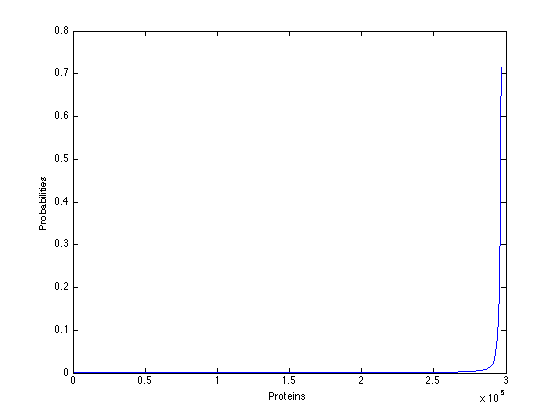
\includegraphics[scale=0.8]{sorted}
\caption{Protein's Probability Distribution}
\label{fig:Protein's Probability Distribution}
\end{figure}
\newpage

To calculate the probabilities of input vectors of different lengths with all other proteins, different parallel programming techniques were applied to improve the performance of our program.
We adopted a distributed memory system approach when parallelizing our program by using the Message Passing Interface(MPI) to broadcast copies of the data to different processes, and distribute the set of proteins among the processes since these do not form any dependencies. In other words, the conditional probability of seeing one protein given the other is not affected by probabilities of other proteins.
Seeing the probability of distribution of the data made it very clear that load balancing techniques have to be applied to achieve a better performance, so we made sure that our program scatters the workload appropriately across different processors. 

We are often interested in building protein networks that involve proteins that are indirectly related to the query protein(s) of interest in addition to those that are directly returned by our program. 
To do this, we extended our program to accept a $`level`$ as a parameter, which resembles how deep we want to  look into the tree of indirectly related proteins. The program first gets all the proteins that are directly related by our query proteins, which will form the first level in our tree rooted by the query protein(s). Then, each of the proteins in the first level is considered these a new query protein. The program keeps running until the level specified by the user is reached, or until no new proteins are found. The number of proteins grows exponentially as we build more levels in our tree, but the program takes into account that a few proteins are mainly abundant by making sure not to redundantly re-compute results for a protein that has been considered a query protein at any point in its execution. This decreases the number of iterations needed for the program to converge. 

Sometimes we are interested in doing our computations across genomes that belong to a certain genus, as opposed to considering the list of all sequenced genomes in our database. Thus, it is useful to be able to constraint the proteins in our search party to a specific genus. This also facilitates answering the question of what proteins are signatures of certain genera. To aid in this, our program takes as an extra parameter a genus of interest, and when parsing the database to fill the input arrays, takes only the set of genomes that belong to that genus into consideration.
To discover proteins that might be specific to a certain genus, or see the differences in the occurrences of proteins across different genera, we developed a program that takes two genera as additional input, finds the common proteins that occur across most of their genomes(the percentage of genomes the proteins must be seen in can also be passed as a parameter), and then outputs the pairs of proteins that maximize the difference between their conditional probabilities in the different genera. We will extend this approach to treat these as signatures specific to the genera. 
One reason we are interested in this is to solve the problem of classifying an unidentified genome and figuring out what genus it belongs to. So to solve this problem, we first extracted 10\% of our database to treat as our training data. Then, using this data, we derived signatures for genera in the following manner: 
For each genus, we computed the occurrences of all its proteins across all the genomes that belong to that genus in our training dataset. Then, we created a signatures database, where each genus is followed by the probability of each of the proteins in that genus. 
We theorized that using these as our signatures would help us classify genomes into their respective genera. To put our theory to a test, we developed a program that, given a certain genome, goes over all the genera in the signatures database, and assigns a score that represents the likelihood of that genome belonging to that genus. The score is computed in a way that can be thought of as a longest common subsequence, where for every protein in the genome, the probability of witnessing that protein in the genus is added to the score, and for every protein that is in the genome but not present in the genus, a penalty is applied. The maximum score is kept across all genera, breaking ties according to the number of proteins that are in common between the genome and the genera, and the genus with the maximum score is returned as the genus to whom our input genome most likely belongs to. We tested this program on the training data, and it achieved 99.8\% accuracy. Furthermore, we tested the program on our whole database of 27,000 genomes, and it achieved 98\% accuracy. It also classified all of unclassified genomes that we had in our database into their corresponding genera with very high confidence scores. 

The problem of discovering novel pathways can be modeled as a very computationally expensive problem. If we limit the set of all possible input vectors of interest to be of length 6, the computational requirements dictated by the problem are enormous. With more than a million different proteins, the set of all possible input vectors of length 6 has cardinality $\binom{1,000,000} {6}$ which is ~ $10^{36}$. If our program takes $10^{-24}$ ms to run as opposed to its current runtime of 700ms for such input length, it would need 30 years to compute all results. If we decide to store results whose probabilities lie above a certain threshold, we still wouldn't get over the fact that to store $10^{-21}$\% of the results we would get, we need 4 PetaBytes. The situation gets much worse when we allow our input vector to have negated variables.

To get around this problem, we followed a different approach. In the paper \cite{9}, the authors identify a metabolic alternative to the classical Mevalonate pathway. To test whether our program can detect any of the two pathways, we used Mevalonate Kinase(MVK) as an input and returned the four proteins with maximum mutual information with MVK. We we thrilled to find that the input MVK together with these four returned proteins form the classical pathway mentioned in the paper. We are currently working on figuring out the FIGFAMs corresponding to the proteins in the alternative pathway to check whether or not our program detects that as well. 
Considering the fact that this may be enough to verify known pathways and detect novel ones, we decided to store the set of all vectors of length 6 representing every possible protein with the 5 other proteins whose mutual information is maximal with it. We are hoping that this could serve as a start to test the possibility of detecting novel pathways by treating these vectors as candidate ones. 
As a side application, seeing that mutual information is returning functionally related proteins, we matched a small subset of proteins whose functions were identified as `hypothetical figfams' to other proteins with well known functions.
\newpage
We are developing a tool that will be deployed as a web service to visualize our results. The tool takes a vector of proteins as an input, along with possible extra parameters like the threshold, distance threshold, specific genus, and the number of levels of indirectly related proteins. It then does the necessary computations and displays the results as a graph. If no threshold was specified, the program returns the 10 proteins whose mutual information with the query protein is maximal and non-zero(to ensure dependence). \\
We use the Mevalonate Kinase pathway mentioned earlier as an example.

\begin{figure}[b!]
\centering
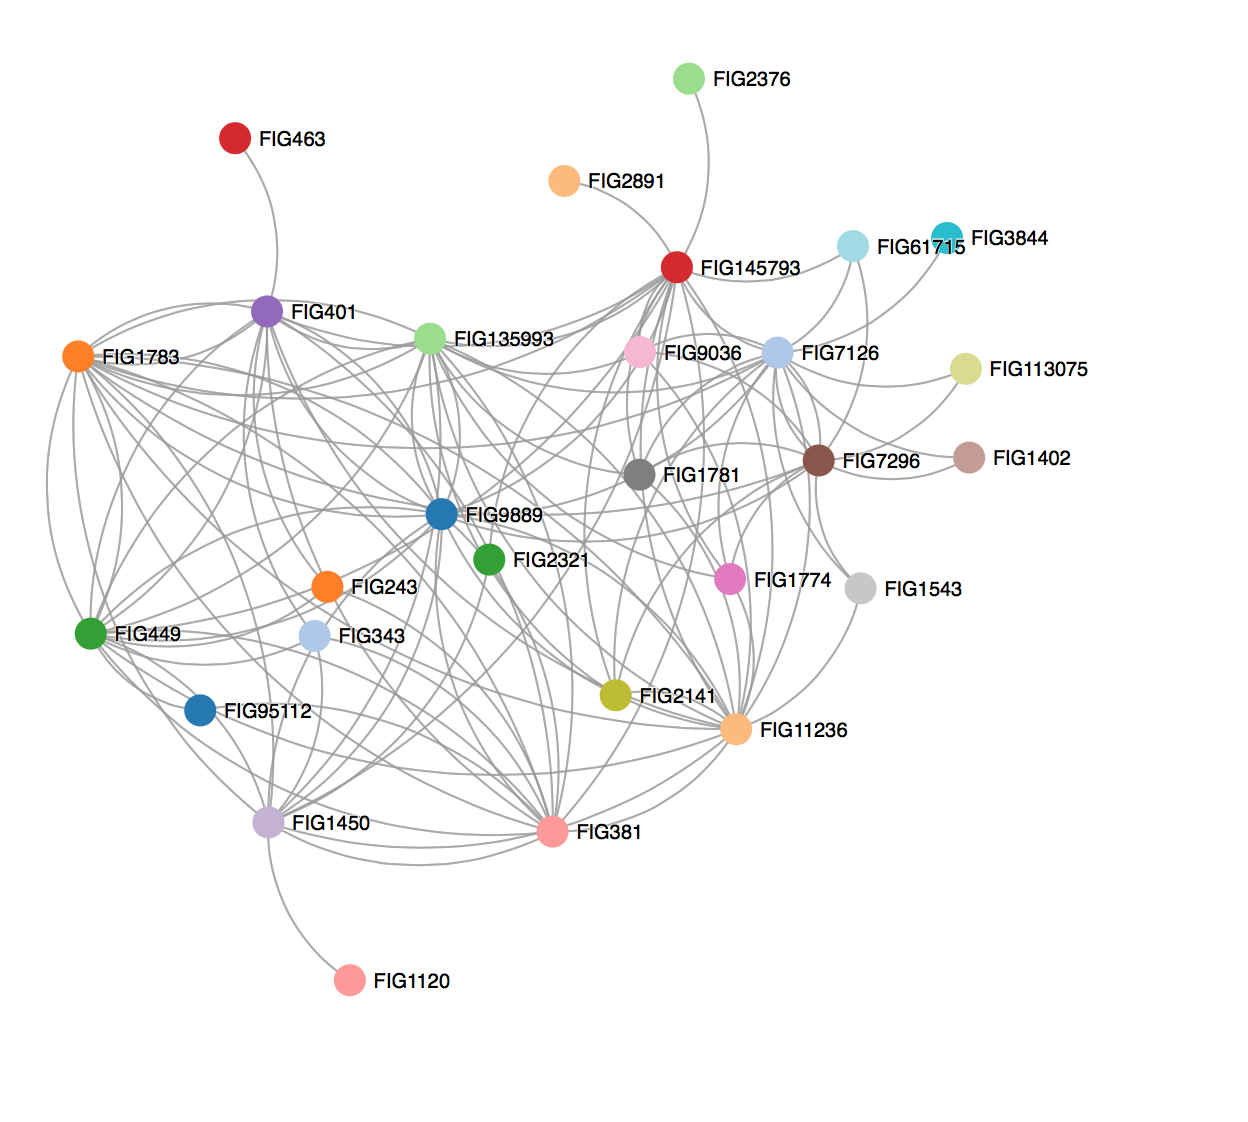
\includegraphics[scale=0.75]{FULLNetwork}
\caption{Protein Network with MVK as input}
\label{fig:Protein Network with MVK as input}
\end{figure}
\newpage
The image above shows the resulting graph when we provide FIG9889(MVK) as a query protein to our program with the  $`level`$ parameter set to 2, and without specifying a threshold, a genus, nor a distance threshold. It thus shows up to 10 related proteins to MVK, and up to 10 related proteins to each of those. 
We use curved edges to better show the connections among the nodes as the graph gets more dense. The nodes of the graph are colored according to the functions of the subsequent proteins. If two proteins have the same function, their nodes will have the same color. The thickness of an edge depends on the value of the correlation between the nodes. Thicker edges mean that the proteins are more strongly correlated(their mutual information is higher) than thinner proteins with thinner edges. 
To check the direct neighborhood of a protein of interest, we can click on a node to highlight it and its immediate neighbors, which would also show the corresponding mutual information value between the highlighted node and its neighbors. As an example, we highlight the FIG9889 node representing MVK, which shows the classical Mevalonate Kinase pathway as part of the highlighted neighbors.
\begin{figure}[b!]
\centering
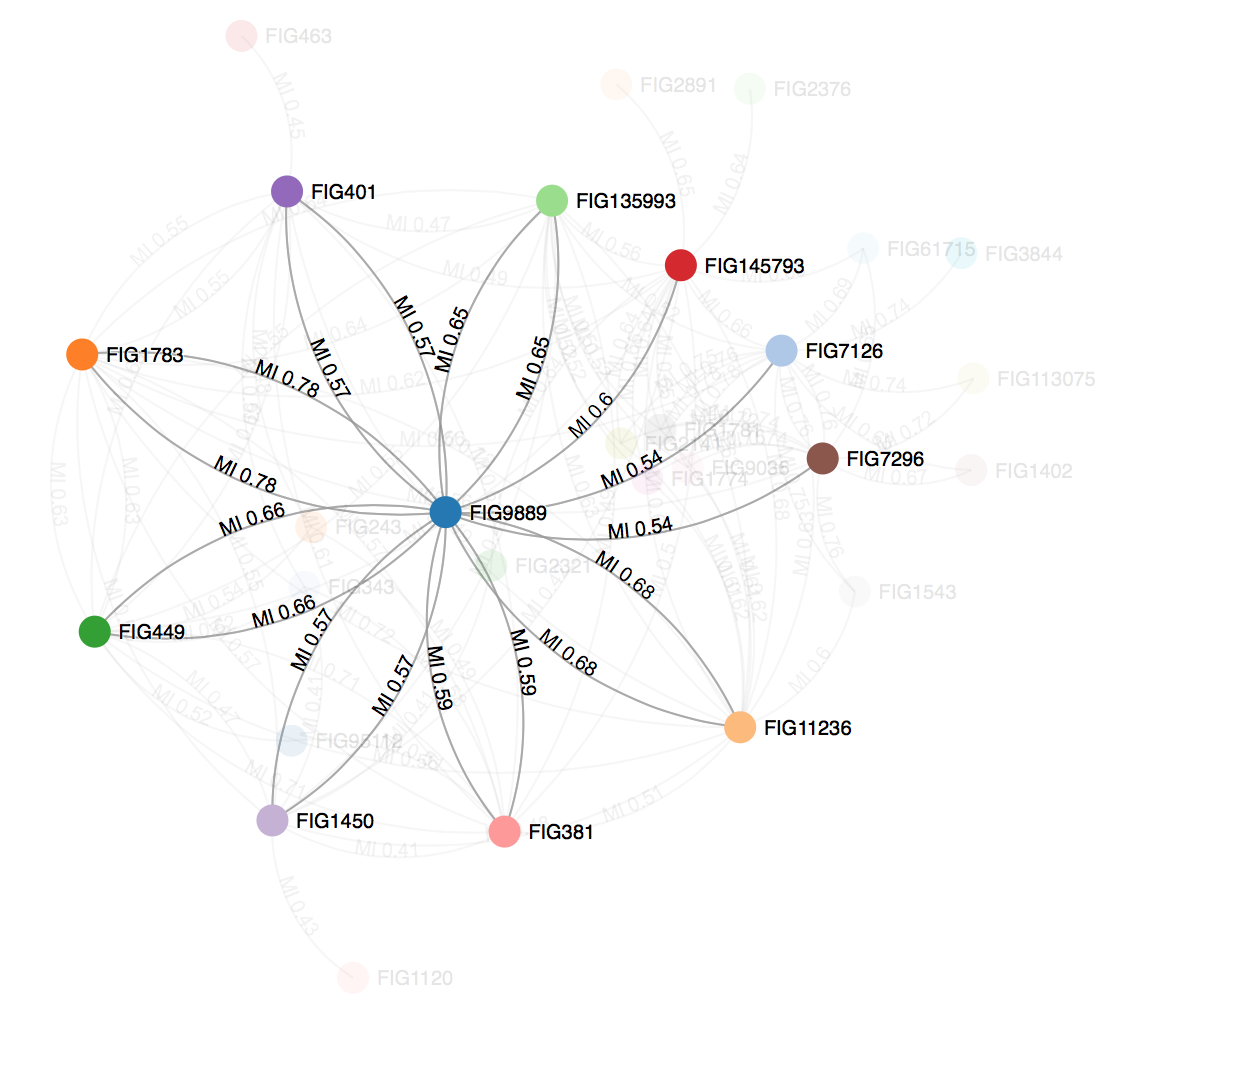
\includegraphics[scale=0.5]{MVKNetwork}
\caption{Protein Network with MVK highlighted}
\label{fig:Protein Network with MVK highlighted}
\end{figure}


\chapter{Concluding Remarks}
We presented a new program for genomic context analysis that extends the functionality of existing tools by allowing the input to be a vector of proteins with the possibility of investigating the absence of proteins and not just their presence. The program returns all proteins that are directly and indirectly related to the query proteins up to a level specified by the user(or until it converges). Aside from the threshold that specifies when two proteins are considered to be potentially related, the user can also specify the maximum distance the proteins can be away from the query protein to be considered potentially related to it. The user may also choose to specify the genus to which the program should limit its computations to when considering the whole set of sequenced genomes in our database. 
We demonstrated the accuracy of our program by using it to detect the known classical pathway of Mevalonate Kinase. We presented the interface of the tool that will incorporate our program's functionality. The tool takes the input from the user and returns the results in the form of a graph representing a protein network.

We also devised an application that  classifies genomes across the classes of genera. The application classified our complete set of genomes in the database with 98\% accuracy. \\
We present fragments of the code we used to develop our program in the appendix. 
\newpage

\begin{appendices}
\chapter{}

\begin{lstlisting}[language=C]

 for (i = 0; i < number_of_genomes; i++) {
        genome_score = 0;
        //record if any of the vector elements have been unlawfully seen
        oops = 0; 
        //index of last protein for this genome
        endg = genome_indices[i]; 
        for (j = startg; j < endg; j++) {
            current_protein = proteins[j];
            if (current_protein >=0) {
            	//count frequency of each protein
                countProteins[current_protein]++; 
                //loop over input vector
                for (k = 0; k < Vlen; k++) { 
               	   //if element of input vector is seen
                    if (current_protein == FFV[k]) { 
                    	//if we are counting its presence
                        if (booleans[k]) { 
                        	   /*count number of elements
	   		    				in vector present in this genome*/
                            genome_score++; 
                        }
                        else { /*if we are counting its absence 
                        	   	the proteins was not supposed
								 to be seen in this form*/
                            oops = 1; 
                        }
                    }
                }
            }
        }
        if (!oops) { //no protein was unlawfully seen
            for (n = 0; n < Vlen; n++) {//loop over input vector
            	//if we are counting this protein's absence
                if (!booleans[n]) { 
                	   // element was rightfully absent from genome
                    genome_score++; 
                }
            }
            //If all input vector was seen in the genome
            if (genome_score == Vlen) { 
                countV++; //count frequency of occurrence of the vector
                //for all other proteins that were in that genome
                for (n = startg; n < endg; n++) { 
                    if (proteins[n] >= 0) {
                        //count frequency of co-occurrence with the vector
                        countVBs[proteins[n]]++; 
                    }
                }
            }
        }
        startg = endg;
    }
\end{lstlisting}
The program loops over all genomes, counting the frequency of occurrence of every protein, the frequency of occurrence of the input vector as a whole, and the frequency of co-occurrence of every vector with the other proteins. 
\newpage

\chapter{}

\begin{lstlisting}[language=C]
    for (i = 0; i < max_protein; i++) {
		//P(V,B): probability of V and protein(call it B)
        probability_VB = ((double)countVBs[i])/number_of_genomes;
        //frequency of co-occurrence of !V(not V) and protein
        countnVBs[i] = countBs[i] - countVBs[i];
        //P(!V,B): probability of !V and protein
        probability_nVB = ((double)countnVBs[i])/number_of_genomes;
        //frequency of co-occurrence of V and !protein
        countVnBs[i] = countV - countVBs[i];
        //P(V,!B): probability of V and !protein
        probability_VnB = ((double)countVnBs[i])/number_of_genomes;
        //frequency of co-occurrence of !V and !protein
        countnVnBs[i] = number_of_genomes - 
        				(countVBs[i] + countnVBs[i] + countVnBs[i]);
        //P(!V,!B): probability of !V and !protein
        probability_nVnB = ((double)countnVnBs[i])/number_of_genomes;

        probability_B_given_V = probability_VB/probability_V; //P(B|V)
        probability_B = ((double)countBs[i])/num_genomes; P(B)
        
        
        
        
        
        
        //Compute different factors in Mutual Information(MI) summation
        if (probability_VB > 0 && probability_V > 0 && probability_B > 0) {
            double px = probability_VB + probability_VnB;
            double py = probability_nVB + probability_VB;
            double denomenator = px * py;
            MI11 = probability_VB * 
            		(log(probability_VB/denomenator)/log(2.0));
        }
        else {
            MI11 = 0;
        }
        if (probability_nVB > 0 && probability_V < 1 && probability_B > 0) {
            double px = probability_nVB + probability_nVnB;
            double py = probability_nVB + probability_VB;
            double denomenator = px * py;
            MI01 = probability_nVB * 
            		(log(probability_nVB/denomenator)/log(2.0));
        }
        else {
            MI01 = 0;
        }
        
        
        
        
        
        
        
        if (probability_VnB > 0 && probability_V > 0 && probability_B < 1) {
            double px = probability_VnB + probability_VB;
            double py = probability_nVnB + probability_VnB;
            double denomenator = px * py;
            MI10 = probability_VnB *
            		 (log(probability_VnB/denomenator)/log(2.0));
        }
        else {
            MI10 = 0;
        }
        if (probability_nVnB > 0 && probability_V < 1 && probability_B < 1) {
            double px = probability_nVnB + probability_nVB;
            double py = probability_nVnB + probability_VnB;
            double denomenator = px * py;
            MI00 = probability_nVnB * 
            		(log(probability_nVnB/denomenator)/log(2.0));
        }
        else {
            MI00 = 0;
        }
        //MI(V,B): Mutual Information of V and B
        MI = MI00 + MI01 + MI10 + MI11; 
}
\end{lstlisting}
The program then checks one protein at a time, calculating its mutual information with the input vector. In the end, it returns the top 10 proteins, or those whose mutual information falls above a certain threshold pre-specified by the user. These proteins will serve as query proteins in subsequent levels if the user chose looking at proteins that are indirectly related to the original query protein. 

\end{appendices}

% Format a LaTeX bibliography
%\makebibliography
\bibliography{thesis}
	\bibliographystyle{plain}

% Figures and tables, if you decide to leave them to the end
%\input{figure}
%\input{table}

\end{document}


